%!TEX root=paper.tex

\subsection{Performance}
\label{sec:perf}

% The \tool also collects information regarding endpoint performance. 
The \perspective{API Performance} visualization perspective presents
an overview of the response times for all the tracked endpoints 
by using a box-and-whiskers plot. 

\Fref{fig:ep} presents such a perspective from our case study which 
was taken in the last quarter of 2017. Several observatrions are 
straightforward: 

\begin{itemize}

  \item The slowest endpoint and the one with the highest variability is \epFeedItemsColor: it retrieves a list of recommended articles for a given user. Since a user can be subscribed to anything from one to three dozen article sources, and since the computation of the difficulty was done in real time, the variability in time among users is likely to be very large. 

  \item In the top three slowest endpoints, but the second most used endpoint in the system (cf. \Fref{fig:aeu}) is \epTranslationsColor. The endpoint is critical being embedded in the interactive loop in the reader applications that rely on the Zeeguu API: a user would tap on a word and receive a translation from this endpoint.
 
\end{itemize}

\begin{figure}[!ht]
 \centering
 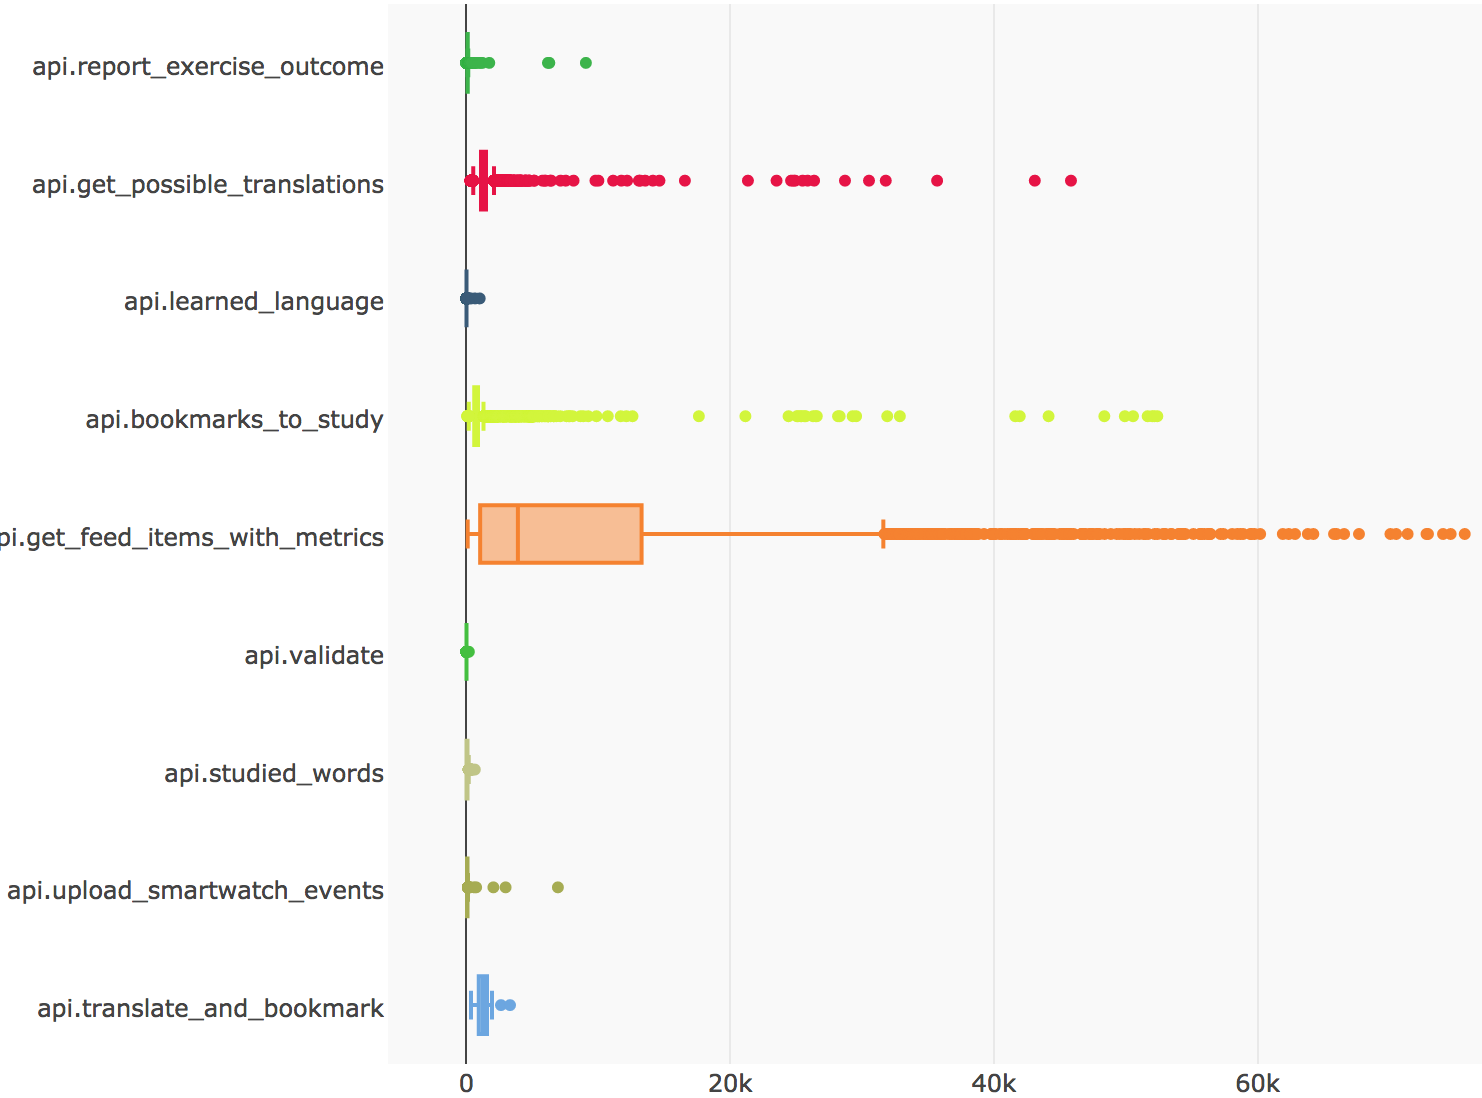
\includegraphics[width=0.85\linewidth]{endpoint_performance_}
 \caption{The response time (in ms) per monitored endpoint view allows for identifying performance variability and balancing issues}
 \label{fig:ep}
\end{figure}

Such a view is important for allocating optimization efforts. In our case study, the API developers started by improving the performance of \epTranslationsColor and then later optimized the performance of \epFeedItemsColor. However, in order to understand the problems of the two endpoints, a big component represents understanding the outliers: because they are many. 


  \subsection{Automated Outlier Detection and Monitoring}
  
  When an API is called from within a highly interactive application (as it is the case with the case study in this paper) 
  of particular interest to the API developers are performance {\em outliers}. 

  Indeed, a translation request that takes three times more than expected can seriously decrease the perceived quality of the application. Thus, identifying, collecting all appropriate data, and diagnosing the root causes of such outliers is especially critical in improving the quality of an application. 
  
  % In the context of the RESTful services support by Flask, this means request serving times that deviate from the average to an unexpected degree. 
  
  For this purpose the \tool tracks for every monitored endpoint a {\em running average} response time value\footnote{\ins{For performance reasons, we assume that the response times for the endpoints are normally distributed. Otherwise, more general density distribution information must be collected in real time.}}. When it detects that a given request is an outlier with respect to this past average running value, it triggers the {\em outlier data collection routine} which stores \ins{extra information} about the current execution environment. A configurable threshold with a default value of $2.5$ times the running average response time is used for this purpose. 

  For every detected outlier request, the \tool collects information about the current Python stack trace, CPU load, memory consumption, request parameters, etc. in order to allow the maintainer to investigate the causes of these exceptionally slow response times. In this way it is possible to get \ins{detailed insight into the operation of the application in the extreme cases without unnecessarily burdening it with logging this information for every request}.


  \begin{figure}[h!]
    \centering
    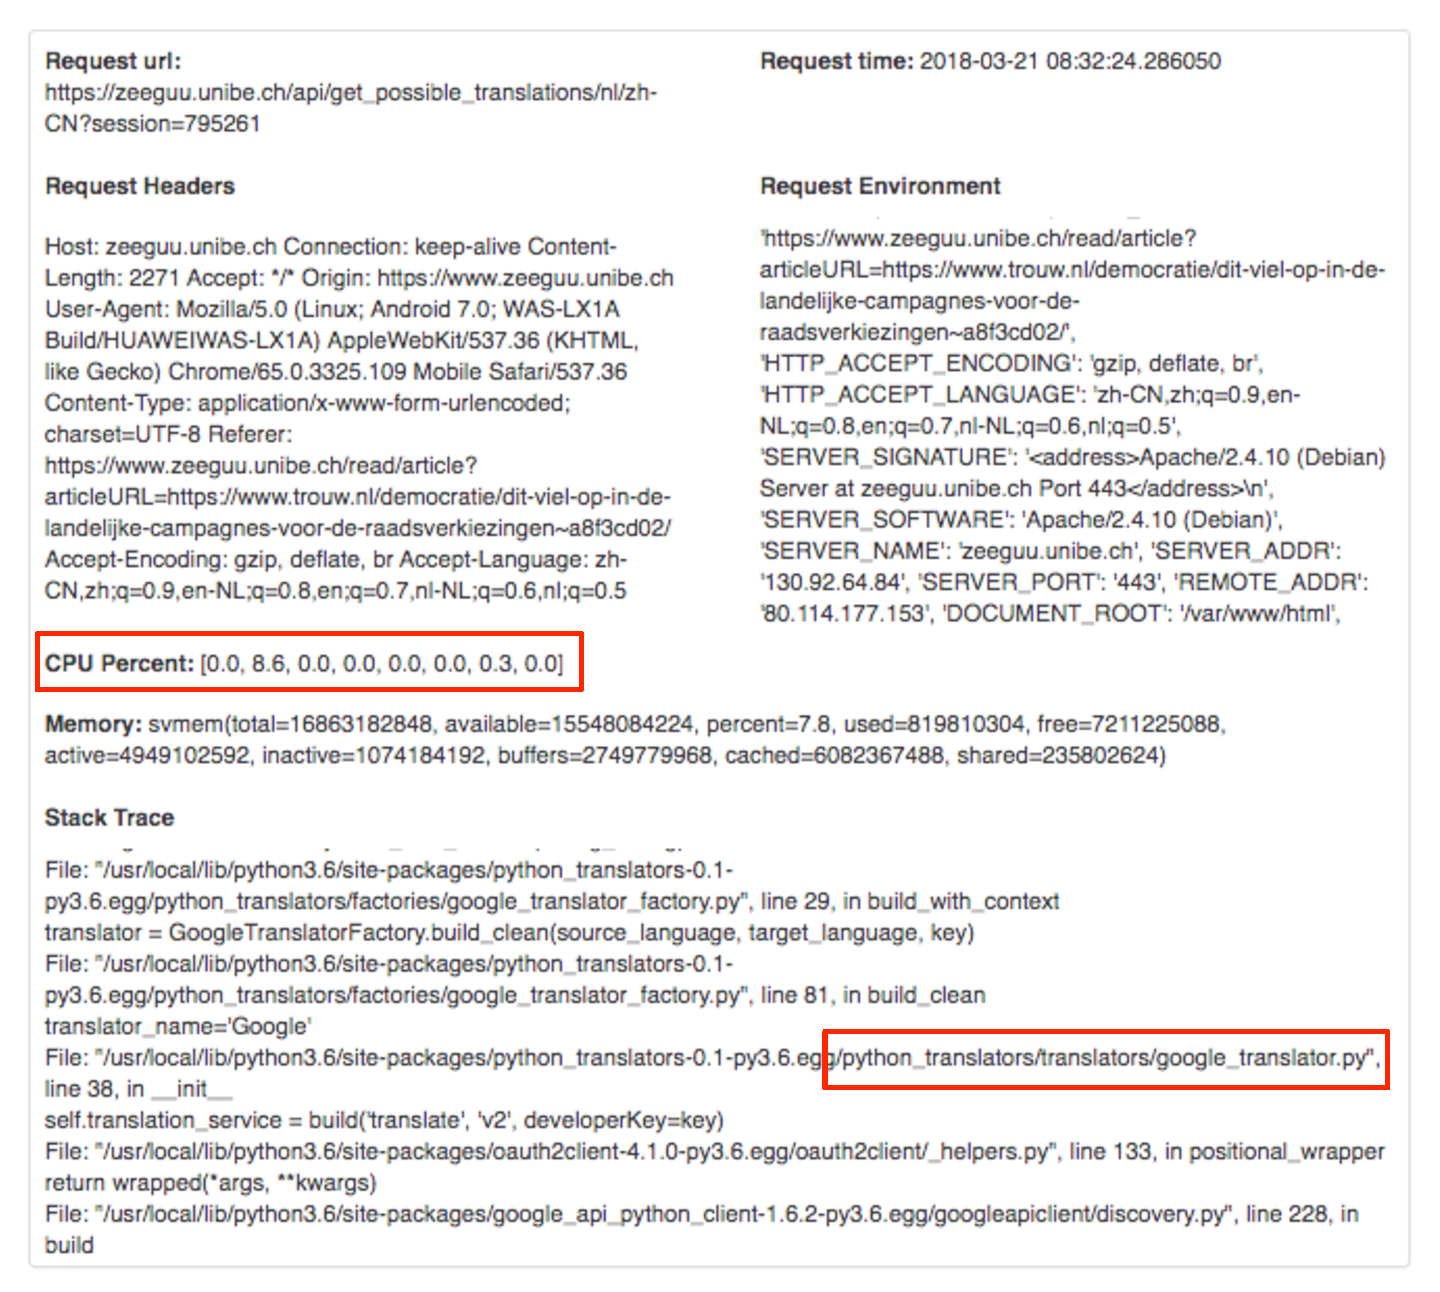
\includegraphics[width=0.9\linewidth]{outlier-annotated}
    \caption{Automatically collected outlier information}
    \label{fig:figure1}
  \end{figure}
  

The bottom panel shows the stack trace. 
In this particular case, it is revealing for the developer to learn that at the time of the stack trace snapshot, the code was in the google\_translator.py: indeed, the system uses as back-end multiple translators, and it has been observed that many of the outliers happen while the system is waiting for the Google translator.

This information has to be corroborated with the observations that neither the memory nor the processor are overloaded at the moment. Thus this functionality in microsoft\_translator is really slow in itself, and this is not a result of the machine being overloaded for example. 









